% ===========================================================================
%  TikuOS — Memory Management: Region Registry
%  Beamer Presentation
% ===========================================================================
\documentclass[aspectratio=169, 10pt]{beamer}

% ---- Theme ----------------------------------------------------------------
\usetheme{Madrid}
\usecolortheme{whale}
\setbeamertemplate{navigation symbols}{}
\setbeamertemplate{footline}{%
  \leavevmode\hbox{%
    \begin{beamercolorbox}[wd=.33\paperwidth,ht=2.5ex,dp=1ex,center]{author in head/foot}%
      \usebeamerfont{author in head/foot}\insertshortauthor
    \end{beamercolorbox}%
    \begin{beamercolorbox}[wd=.34\paperwidth,ht=2.5ex,dp=1ex,center]{title in head/foot}%
      \usebeamerfont{title in head/foot}\insertshorttitle
    \end{beamercolorbox}%
    \begin{beamercolorbox}[wd=.33\paperwidth,ht=2.5ex,dp=1ex,right]{date in head/foot}%
      \usebeamerfont{date in head/foot}\insertshortdate{}\hspace*{2em}%
      \insertframenumber{}/\inserttotalframenumber\hspace*{2ex}
    \end{beamercolorbox}}%
  \vskip0pt%
}

% ---- Packages -------------------------------------------------------------
\usepackage{listings}
\usepackage{graphicx}
\usepackage{hyperref}
\usepackage{booktabs}
\usepackage{multirow}
\usepackage{tikz}
\usetikzlibrary{arrows.meta, positioning, shapes.geometric, calc, decorations.pathreplacing}

% ---- Code listing style ---------------------------------------------------
\lstset{
  basicstyle=\ttfamily\scriptsize,
  keywordstyle=\color{blue}\bfseries,
  commentstyle=\color{gray},
  stringstyle=\color{red!70!black},
  showstringspaces=false,
  breaklines=true,
  frame=single,
  rulecolor=\color{black!30},
  backgroundcolor=\color{blue!3},
  tabsize=4,
}
\lstdefinestyle{cstyle}{
  language=C,
  morekeywords={uint8_t,uint16_t,uint32_t,uintptr_t,
                tiku_mem_region_t,tiku_mem_region_type_t,
                tiku_mem_claimed_t,tiku_mem_err_t,tiku_mem_arch_size_t,
                tiku_arena_t,tiku_persist_store_t,
                TIKU_MEM_REGION_SRAM,TIKU_MEM_REGION_NVM,
                TIKU_MEM_REGION_PERIPHERAL,TIKU_MEM_REGION_FLASH,
                TIKU_MEM_OK,TIKU_MEM_ERR_INVALID,TIKU_MEM_ERR_FULL,
                TIKU_MEM_ERR_NOT_FOUND,TIKU_REGION_MAX_REGIONS,
                TIKU_REGION_MAX_CLAIMS,NULL},
}
\lstdefinestyle{bashstyle}{
  language=bash,
  morekeywords={sudo,apt,make,gcc},
}

% ---- Metadata -------------------------------------------------------------
\title[TikuOS Region]{TikuOS Memory Region Registry}
\subtitle{Simple. Ubiquitous. Intelligence, Everywhere.}
\author[Ambuj Varshney]{Ambuj Varshney \\ \texttt{ambuj@tiku-os.org}}
\date{\today}

% ===========================================================================
\begin{document}

% ---------------------------------------------------------------------------
\begin{frame}
\titlepage
\end{frame}

% ---------------------------------------------------------------------------
\begin{frame}{Outline}
\tableofcontents
\end{frame}

% ===========================================================================
\section{Why a Region Registry?}
% ===========================================================================

\begin{frame}{The Problem: Wrong Buffer Placement}
\begin{columns}[T]
\begin{column}{0.48\textwidth}
\textbf{Without region validation:}
\begin{itemize}
  \item Arena buffer accidentally placed in FRAM
  \item Persistent store backed by volatile SRAM
  \item Two subsystems sharing the same buffer
  \item Stack-allocated buffer passed to arena create
  \item All silent, all diagnosed at 3\,AM
\end{itemize}

\vspace{0.5em}
\begin{alertblock}{Silent Misplacement}
On a microcontroller with SRAM and FRAM in the same flat
address space, nothing prevents you from creating an arena
in FRAM or a persistent store in SRAM.  The code compiles,
the system boots, and the bug manifests as unexplained data
corruption --- hours or days later.
\end{alertblock}
\end{column}

\begin{column}{0.48\textwidth}
\textbf{TikuOS region registry:}
\begin{itemize}
  \item Boot-time memory map from platform HAL
  \item \texttt{contains()} validates buffer type
  \item Arena create rejects non-SRAM buffers
  \item Persist register rejects non-NVM buffers
  \item \texttt{claim()} detects overlapping buffers
  \item \texttt{get\_type()} for diagnostics
\end{itemize}

\vspace{0.5em}
\begin{block}{Fail Fast at Init}
The region registry catches buffer placement errors at
\texttt{create()} / \texttt{register()} time --- before the
system runs.  The cost is a few linear scans during boot;
the hot path is untouched.
\end{block}
\end{column}
\end{columns}
\end{frame}

% ---------------------------------------------------------------------------
\begin{frame}{MSP430 Memory Map: Why Types Matter}
\begin{center}
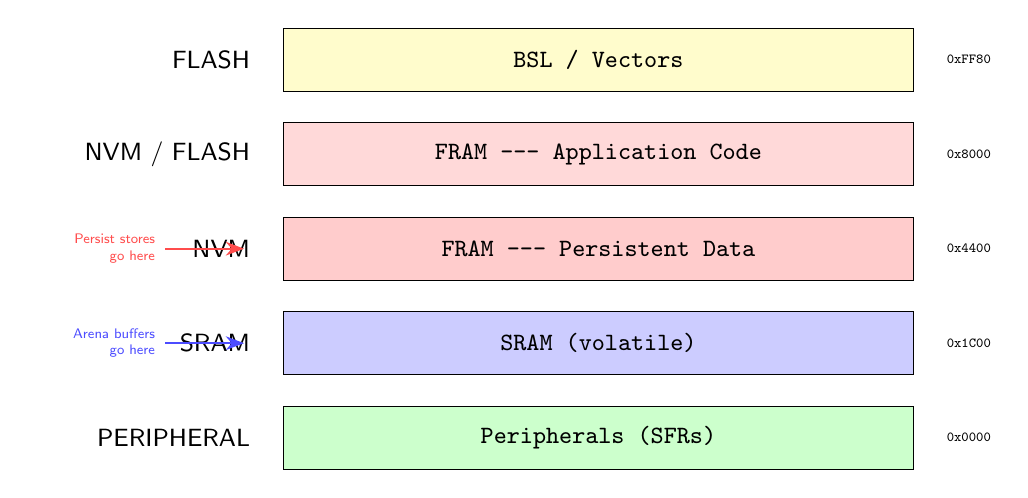
\begin{tikzpicture}[
    region/.style={draw, minimum width=8cm, minimum height=0.8cm,
                   font=\small\ttfamily, align=center},
    label/.style={font=\small\sffamily, anchor=east},
    addr/.style={font=\tiny\ttfamily, anchor=west},
    >=Stealth
  ]
  % Memory regions (bottom to top = low to high address)
  \node[region, fill=green!20] (periph) at (0, 0) {Peripherals (SFRs)};
  \node[region, fill=blue!20]  (sram)   at (0, 1.2) {SRAM (volatile)};
  \node[region, fill=red!20]   (fram1)  at (0, 2.4) {FRAM --- Persistent Data};
  \node[region, fill=red!15]   (fram2)  at (0, 3.6) {FRAM --- Application Code};
  \node[region, fill=yellow!20](bsl)    at (0, 4.8) {BSL / Vectors};

  % Addresses
  \node[addr] at (4.3, 0)   {0x0000};
  \node[addr] at (4.3, 1.2) {0x1C00};
  \node[addr] at (4.3, 2.4) {0x4400};
  \node[addr] at (4.3, 3.6) {0x8000};
  \node[addr] at (4.3, 4.8) {0xFF80};

  % Type annotations
  \node[label] at (-4.3, 0)   {PERIPHERAL};
  \node[label] at (-4.3, 1.2) {SRAM};
  \node[label] at (-4.3, 2.4) {NVM};
  \node[label] at (-4.3, 3.6) {NVM / FLASH};
  \node[label] at (-4.3, 4.8) {FLASH};

  % Annotations
  \draw[->, thick, blue!70] (-5.5, 1.2) -- (-4.5, 1.2)
    node[pos=0, anchor=east, font=\tiny\sffamily, text width=1.5cm, align=right]
    {Arena buffers go here};
  \draw[->, thick, red!70] (-5.5, 2.4) -- (-4.5, 2.4)
    node[pos=0, anchor=east, font=\tiny\sffamily, text width=1.5cm, align=right]
    {Persist stores go here};
\end{tikzpicture}
\end{center}

\vspace{0.3em}
\begin{block}{Flat Address Space, Different Rules}
All regions share one 16-bit address space. A pointer to \texttt{0x1D00}
(SRAM) looks identical to a pointer to \texttt{0x4500} (FRAM). Only the
region registry knows which is which.
\end{block}
\end{frame}

% ===========================================================================
\section{Architecture \& Data Structures}
% ===========================================================================

\begin{frame}[fragile]{Region Types \& Descriptors (kernel/memory/tiku\_mem.h)}
\begin{columns}[T]
\begin{column}{0.48\textwidth}
\begin{lstlisting}[style=cstyle, title={Region type enum}]
typedef enum {
    TIKU_MEM_REGION_SRAM,
    TIKU_MEM_REGION_NVM,
    TIKU_MEM_REGION_PERIPHERAL,
    TIKU_MEM_REGION_FLASH
} tiku_mem_region_type_t;
\end{lstlisting}

\begin{lstlisting}[style=cstyle, title={Region descriptor}]
typedef struct tiku_mem_region {
    const uint8_t          *base;
    tiku_mem_arch_size_t    size;
    tiku_mem_region_type_t  type;
} tiku_mem_region_t;
\end{lstlisting}
\end{column}

\begin{column}{0.48\textwidth}
\begin{lstlisting}[style=cstyle, title={Claimed region (overlap tracking)}]
typedef struct {
    const uint8_t          *base;
    tiku_mem_arch_size_t    size;
    uint8_t                 owner_id;
} tiku_mem_claimed_t;
\end{lstlisting}

\vspace{0.5em}
\begin{block}{Design Choices}
\begin{itemize}
  \item Struct tag \texttt{tiku\_mem\_region} enables forward
        declaration in the HAL header
  \item \texttt{const uint8\_t *base} --- region table is
        read-only (lives in flash)
  \item \texttt{owner\_id} links claims to subsystems
        for diagnostic output
\end{itemize}
\end{block}
\end{column}
\end{columns}
\end{frame}

% ---------------------------------------------------------------------------
\begin{frame}[fragile]{Internal State (kernel/memory/tiku\_region.c)}
\begin{lstlisting}[style=cstyle]
/** Pointer to platform-provided region table (lives in flash) */
static const tiku_mem_region_t *region_table;

/** Number of entries in the region table */
static tiku_mem_arch_size_t region_count;

/** Claimed region tracking array (lives in SRAM) */
static tiku_mem_claimed_t claimed[TIKU_REGION_MAX_CLAIMS];

/** Number of active claims */
static tiku_mem_arch_size_t claimed_count;
\end{lstlisting}

\vspace{0.3em}
\begin{columns}[T]
\begin{column}{0.48\textwidth}
\begin{block}{Zero-Copy Region Table}
\texttt{region\_table} is a \emph{pointer} to the platform's const
array --- no copy is made.  The table lives in flash; we just store
its address and length.
\end{block}
\end{column}
\begin{column}{0.48\textwidth}
\begin{block}{Configurable Limits}
\texttt{TIKU\_REGION\_MAX\_REGIONS} (default 10) and
\texttt{TIKU\_REGION\_MAX\_CLAIMS} (default 16) are overridable
at compile time for platforms with more complex memory maps.
\end{block}
\end{column}
\end{columns}
\end{frame}

% ===========================================================================
\section{Platform Layering}
% ===========================================================================

\begin{frame}[fragile]{Three-Layer Architecture}
\begin{center}
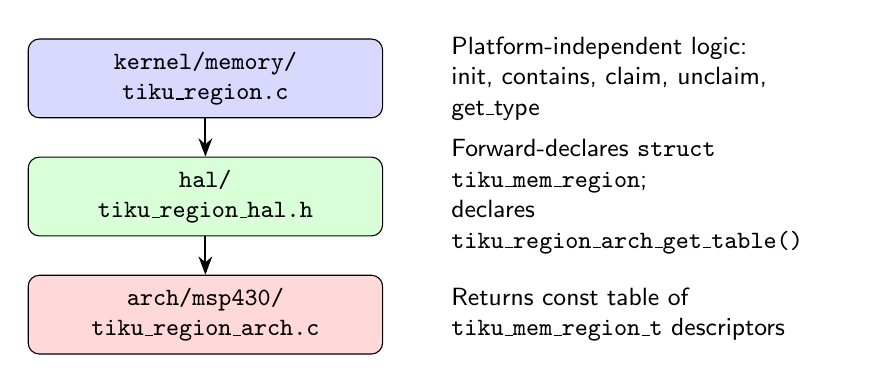
\begin{tikzpicture}[
    box/.style={draw, rounded corners, minimum width=4.5cm, minimum height=1cm,
                font=\small\ttfamily, align=center},
    arrow/.style={->, thick, >=Stealth},
    label/.style={font=\small\sffamily, text width=5cm, align=left}
  ]
  \node[box, fill=blue!15] (kernel) at (0, 3)
    {kernel/memory/\\tiku\_region.c};
  \node[box, fill=green!15] (hal) at (0, 1.5)
    {hal/\\tiku\_region\_hal.h};
  \node[box, fill=red!15] (arch) at (0, 0)
    {arch/msp430/\\tiku\_region\_arch.c};

  \draw[arrow] (kernel) -- (hal);
  \draw[arrow] (hal) -- (arch);

  \node[label, anchor=west] at (3, 3) {Platform-independent logic:\\
    init, contains, claim, unclaim, get\_type};
  \node[label, anchor=west] at (3, 1.5) {Forward-declares \texttt{struct tiku\_mem\_region};\\
    declares \texttt{tiku\_region\_arch\_get\_table()}};
  \node[label, anchor=west] at (3, 0) {Returns const table of\\
    \texttt{tiku\_mem\_region\_t} descriptors};
\end{tikzpicture}
\end{center}

\vspace{0.3em}
\begin{block}{Same HAL Pattern as MPU and Arena}
The region registry follows the same three-layer pattern:
kernel logic calls a HAL-declared function, and the platform
arch layer provides the implementation.  Porting to a new MCU
means writing one function --- \texttt{tiku\_region\_arch\_get\_table()}.
\end{block}
\end{frame}

% ---------------------------------------------------------------------------
\begin{frame}[fragile]{HAL Interface \& Forward Declaration}
\begin{columns}[T]
\begin{column}{0.48\textwidth}
\begin{lstlisting}[style=cstyle, title={hal/tiku\_region\_hal.h}]
#ifndef TIKU_REGION_HAL_H_
#define TIKU_REGION_HAL_H_

#include <stdint.h>
#include "hal/tiku_mem_hal.h"

/* Full definition in tiku_mem.h */
struct tiku_mem_region;

/**
 * Return the platform's memory
 * region table.
 */
const struct tiku_mem_region *
tiku_region_arch_get_table(
    tiku_mem_arch_size_t *count);

#endif /* TIKU_REGION_HAL_H_ */
\end{lstlisting}
\end{column}

\begin{column}{0.48\textwidth}
\begin{lstlisting}[style=cstyle, title={MSP430 arch implementation}]
static const tiku_mem_region_t
    msp430_region_table[] =
{
    { (const uint8_t *)0x1C00,
      TIKU_DEVICE_SRAM_SIZE,
      TIKU_MEM_REGION_SRAM },

    { (const uint8_t *)0x4400,
      TIKU_DEVICE_FRAM_SIZE,
      TIKU_MEM_REGION_NVM },
};

const struct tiku_mem_region *
tiku_region_arch_get_table(
    tiku_mem_arch_size_t *count)
{
    *count = 2;
    return msp430_region_table;
}
\end{lstlisting}
\end{column}
\end{columns}

\vspace{0.3em}
\begin{alertblock}{Forward Declaration Avoids Circular Include}
\texttt{tiku\_region\_hal.h} uses a forward \texttt{struct tiku\_mem\_region}
declaration so it does not need to include \texttt{tiku\_mem.h}. The full
typedef is in \texttt{tiku\_mem.h} which includes the HAL header ---
no circular dependency.
\end{alertblock}
\end{frame}

% ===========================================================================
\section{API Reference}
% ===========================================================================

\begin{frame}[fragile]{tiku\_region\_init()}
\begin{lstlisting}[style=cstyle]
tiku_mem_err_t tiku_region_init(const tiku_mem_region_t *table,
                                 tiku_mem_arch_size_t count);
\end{lstlisting}

\begin{lstlisting}[style=cstyle, title={kernel/memory/tiku\_region.c}]
tiku_mem_err_t tiku_region_init(const tiku_mem_region_t *table,
                                 tiku_mem_arch_size_t count) {
    /* Validate arguments */
    if (table == NULL || count == 0 || count > TIKU_REGION_MAX_REGIONS)
        return TIKU_MEM_ERR_INVALID;

    /* Check for pairwise overlaps in the platform's region table */
    for (i = 0; i < count; i++)
        for (j = i + 1; j < count; j++)
            if (ranges_overlap(table[i].base, table[i].size,
                               table[j].base, table[j].size))
                return TIKU_MEM_ERR_INVALID;

    region_table = table;   /* store pointer (no copy) */
    region_count = count;
    /* Zero the claimed regions array */
    ...
    return TIKU_MEM_OK;
}
\end{lstlisting}

\begin{block}{Boot Sequence}
\texttt{tiku\_mem\_init()} calls \texttt{tiku\_region\_init()} \emph{first},
before \texttt{tiku\_mpu\_init()}.  The region registry must be ready before
any arena or persist subsystem tries to validate its buffer.
\end{block}
\end{frame}

% ---------------------------------------------------------------------------
\begin{frame}[fragile]{tiku\_region\_contains()}
\begin{lstlisting}[style=cstyle]
tiku_mem_err_t tiku_region_contains(const uint8_t *ptr,
                                     tiku_mem_arch_size_t size,
                                     tiku_mem_region_type_t expected_type);
\end{lstlisting}

\begin{lstlisting}[style=cstyle, title={kernel/memory/tiku\_region.c}]
tiku_mem_err_t tiku_region_contains(const uint8_t *ptr,
                                     tiku_mem_arch_size_t size,
                                     tiku_mem_region_type_t expected_type) {
    if (ptr == NULL || size == 0) return 0;

    range_start = (uintptr_t)ptr;
    range_end   = range_start + (uintptr_t)size;
    if (range_end < range_start) return 0;  /* overflow check */

    for (i = 0; i < region_count; i++) {
        if (region_table[i].type != expected_type) continue;
        reg_start = (uintptr_t)region_table[i].base;
        reg_end   = reg_start + (uintptr_t)region_table[i].size;
        if (range_start >= reg_start && range_end <= reg_end) return 1;
    }
    return 0;
}
\end{lstlisting}

\begin{columns}[T]
\begin{column}{0.48\textwidth}
\begin{alertblock}{Why \texttt{uintptr\_t}?}
Comparing pointers to different objects is undefined behavior
in C.  Casting to \texttt{uintptr\_t} gives well-defined integer
comparison across all memory regions.
\end{alertblock}
\end{column}
\begin{column}{0.48\textwidth}
\begin{alertblock}{16-bit Overflow Check}
On MSP430, \texttt{ptr + size} can wrap past \texttt{0xFFFF}.
The \texttt{range\_end < range\_start} guard catches this before
it fools the containment check.
\end{alertblock}
\end{column}
\end{columns}
\end{frame}

% ---------------------------------------------------------------------------
\begin{frame}[fragile]{tiku\_region\_claim() / tiku\_region\_unclaim()}
\begin{columns}[T]
\begin{column}{0.48\textwidth}
\begin{lstlisting}[style=cstyle, title={Claim --- register ownership}]
tiku_mem_err_t tiku_region_claim(
    const uint8_t *ptr,
    tiku_mem_arch_size_t size,
    uint8_t owner_id)
{
    if (ptr == NULL || size == 0)
        return TIKU_MEM_ERR_INVALID;

    /* Must be in a declared region */
    if (!region_is_known(ptr, size))
        return TIKU_MEM_ERR_INVALID;

    /* Check overlap with claims */
    for (i = 0; i < MAX_CLAIMS; i++)
        if (claimed[i].size != 0 &&
            ranges_overlap(...))
            return TIKU_MEM_ERR_INVALID;

    /* Store in first empty slot */
    claimed[i] = { ptr, size, id };
    return TIKU_MEM_OK;
}
\end{lstlisting}
\end{column}

\begin{column}{0.48\textwidth}
\begin{lstlisting}[style=cstyle, title={Unclaim --- release ownership}]
tiku_mem_err_t tiku_region_unclaim(
    const uint8_t *ptr)
{
    if (ptr == NULL)
        return TIKU_MEM_ERR_NOT_FOUND;

    for (i = 0; i < MAX_CLAIMS; i++) {
        if (claimed[i].size != 0 &&
            (uintptr_t)claimed[i].base
            == (uintptr_t)ptr) {
            claimed[i] = { 0 };
            claimed_count--;
            return TIKU_MEM_OK;
        }
    }
    return TIKU_MEM_ERR_NOT_FOUND;
}
\end{lstlisting}

\vspace{0.3em}
\begin{block}{Three Validations}
\texttt{claim()} verifies:
\begin{enumerate}
  \item Range is in known memory
  \item No overlap with existing claims
  \item Claim table not full
\end{enumerate}
\end{block}
\end{column}
\end{columns}
\end{frame}

% ---------------------------------------------------------------------------
\begin{frame}[fragile]{tiku\_region\_get\_type()}
\begin{lstlisting}[style=cstyle]
tiku_mem_err_t tiku_region_get_type(const uint8_t *ptr,
                                     tiku_mem_region_type_t *out_type);
\end{lstlisting}

\begin{lstlisting}[style=cstyle, title={kernel/memory/tiku\_region.c}]
tiku_mem_err_t tiku_region_get_type(const uint8_t *ptr,
                                     tiku_mem_region_type_t *out_type) {
    if (ptr == NULL || out_type == NULL) return TIKU_MEM_ERR_NOT_FOUND;

    addr = (uintptr_t)ptr;
    for (i = 0; i < region_count; i++) {
        reg_start = (uintptr_t)region_table[i].base;
        reg_end   = reg_start + (uintptr_t)region_table[i].size;
        if (addr >= reg_start && addr < reg_end) {
            *out_type = region_table[i].type;
            return TIKU_MEM_OK;
        }
    }
    return TIKU_MEM_ERR_NOT_FOUND;
}
\end{lstlisting}

\vspace{0.3em}
\begin{block}{Diagnostic Utility}
\texttt{get\_type()} looks up a single address and returns which region
type it belongs to. Useful for debug printing (``this pointer is in
SRAM / NVM / peripheral space'') and for runtime assertions in
development builds.
\end{block}
\end{frame}

% ---------------------------------------------------------------------------
\begin{frame}[fragile]{Private Helper: ranges\_overlap()}
\begin{lstlisting}[style=cstyle, title={kernel/memory/tiku\_region.c}]
static int ranges_overlap(const uint8_t *a_base, tiku_mem_arch_size_t a_size,
                            const uint8_t *b_base, tiku_mem_arch_size_t b_size)
{
    uintptr_t a_start = (uintptr_t)a_base;
    uintptr_t a_end   = a_start + (uintptr_t)a_size;
    uintptr_t b_start = (uintptr_t)b_base;
    uintptr_t b_end   = b_start + (uintptr_t)b_size;

    return (a_start < b_end) && (b_start < a_end);
}
\end{lstlisting}

\vspace{0.5em}
\begin{columns}[T]
\begin{column}{0.48\textwidth}
\begin{block}{Classic Interval Overlap Test}
Two half-open intervals $[a, a{+}s)$ and $[b, b{+}s)$ overlap
if and only if $a < b\_\text{end}$ AND $b < a\_\text{end}$.
This is the standard algorithm from computational geometry.
\end{block}
\end{column}
\begin{column}{0.48\textwidth}
\begin{block}{Used Twice}
\begin{enumerate}
  \item \textbf{Init:} Rejects overlapping platform regions
  \item \textbf{Claim:} Detects conflicting buffer assignments
\end{enumerate}
Adjacent ranges (\texttt{a\_end == b\_start}) do \textbf{not}
overlap --- this is correct because half-open intervals exclude
the end point.
\end{block}
\end{column}
\end{columns}
\end{frame}

% ===========================================================================
\section{Integration}
% ===========================================================================

\begin{frame}[fragile]{Integration into Existing Subsystems}
\begin{columns}[T]
\begin{column}{0.48\textwidth}
\begin{lstlisting}[style=cstyle, title={tiku\_arena\_create() --- added check}]
tiku_mem_err_t tiku_arena_create(
    tiku_arena_t *arena,
    uint8_t *buf,
    tiku_mem_arch_size_t size,
    uint8_t id)
{
    /* NULL checks ... */

    /* NEW: buffer must be in SRAM */
    if (!tiku_region_contains(buf, size,
            TIKU_MEM_REGION_SRAM))
        return TIKU_MEM_ERR_INVALID;

    /* NEW: claim for overlap detect */
    tiku_region_claim(buf, size, id);

    /* ... existing init code ... */
}
\end{lstlisting}
\end{column}

\begin{column}{0.48\textwidth}
\begin{lstlisting}[style=cstyle, title={tiku\_persist\_register() --- added check}]
tiku_mem_err_t tiku_persist_register(
    tiku_persist_store_t *store,
    uint8_t *fram_buf,
    tiku_mem_arch_size_t capacity,
    ...)
{
    /* NULL checks ... */

    /* NEW: buffer must be in NVM */
    if (!tiku_region_contains(
            fram_buf, capacity,
            TIKU_MEM_REGION_NVM))
        return TIKU_MEM_ERR_INVALID;

    /* ... existing init code ... */
}
\end{lstlisting}

\vspace{0.3em}
\begin{alertblock}{Two Lines per Subsystem}
Each allocator gains a \texttt{contains()} guard and an optional
\texttt{claim()}. Minimal code change, maximum safety.
\end{alertblock}
\end{column}
\end{columns}
\end{frame}

% ---------------------------------------------------------------------------
\begin{frame}[fragile]{Boot Sequence with Region Registry}
\begin{center}
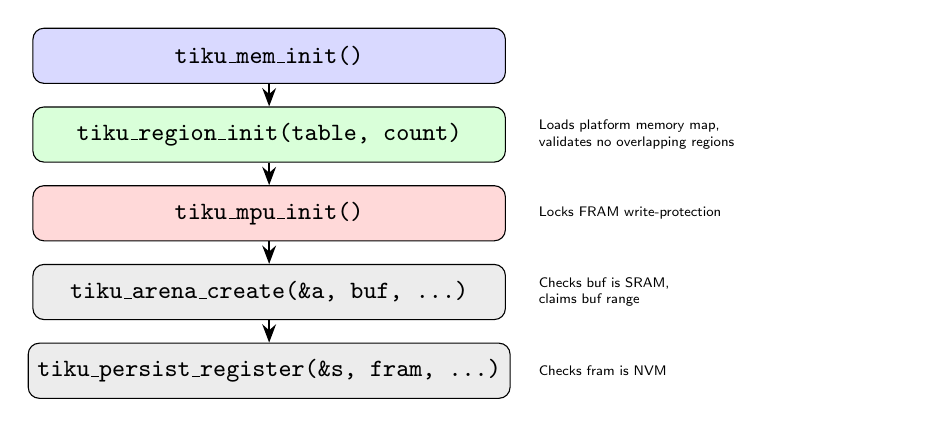
\begin{tikzpicture}[
    bootstep/.style={draw, rounded corners, minimum width=6cm, minimum height=0.7cm,
                     font=\small\ttfamily, align=center},
    arrow/.style={->, thick, >=Stealth},
    note/.style={font=\tiny\sffamily, text width=4.5cm, align=left}
  ]
  \node[bootstep, fill=blue!15] (init) at (0, 4) {tiku\_mem\_init()};
  \node[bootstep, fill=green!15] (region) at (0, 3) {tiku\_region\_init(table, count)};
  \node[bootstep, fill=red!15] (mpu) at (0, 2) {tiku\_mpu\_init()};
  \node[bootstep, fill=gray!15] (arena) at (0, 1) {tiku\_arena\_create(\&a, buf, ...)};
  \node[bootstep, fill=gray!15] (persist) at (0, 0) {tiku\_persist\_register(\&s, fram, ...)};

  \draw[arrow] (init) -- (region);
  \draw[arrow] (region) -- (mpu);
  \draw[arrow] (mpu) -- (arena);
  \draw[arrow] (arena) -- (persist);

  \node[note, anchor=west] at (3.3, 3) {Loads platform memory map,\\validates no overlapping regions};
  \node[note, anchor=west] at (3.3, 2) {Locks FRAM write-protection};
  \node[note, anchor=west] at (3.3, 1) {Checks buf is SRAM,\\claims buf range};
  \node[note, anchor=west] at (3.3, 0) {Checks fram is NVM};
\end{tikzpicture}
\end{center}

\vspace{0.3em}
\begin{block}{Order Matters}
Region init runs first so that arena and persist can validate their
buffers.  MPU init runs second so that FRAM is write-protected before
any application code.  Arena and persist run last, using both the region
registry (for type checking) and the MPU (for write protection).
\end{block}
\end{frame}

% ===========================================================================
\section{Usage Examples}
% ===========================================================================

\begin{frame}[fragile]{Example 1: The Bug Region Registry Catches}
\begin{columns}[T]
\begin{column}{0.48\textwidth}
\begin{lstlisting}[style=cstyle, title={Bug: arena in FRAM}]
/* Developer places arena buffer in
   FRAM by mistake (wrong section) */
static uint8_t __attribute__((
    section(".persistent")))
    scratch[128] = {0};

static tiku_arena_t arena;

void init(void) {
    /* Without region check:
       silently creates arena in FRAM.
       Every alloc writes to NVM --
       wears out FRAM, wastes cycles,
       data persists unexpectedly. */
    tiku_arena_create(&arena,
        scratch, 128, 1);
}
\end{lstlisting}
\end{column}

\begin{column}{0.48\textwidth}
\begin{lstlisting}[style=cstyle, title={With region registry}]
void init(void) {
    tiku_mem_err_t err;
    err = tiku_arena_create(&arena,
        scratch, 128, 1);

    /* tiku_region_contains(scratch,
       128, TIKU_MEM_REGION_SRAM)
       returns 0 --- scratch is in
       NVM, not SRAM!

       arena_create returns
       TIKU_MEM_ERR_INVALID.

       Bug caught at init time. */

    if (err != TIKU_MEM_OK)
        fault_handler("bad arena buf");
}
\end{lstlisting}

\begin{alertblock}{Caught Immediately}
Instead of silent FRAM wear, the error is reported
at boot.  No runtime corruption to debug.
\end{alertblock}
\end{column}
\end{columns}
\end{frame}

% ---------------------------------------------------------------------------
\begin{frame}[fragile]{Example 2: Overlapping Buffer Detection}
\begin{lstlisting}[style=cstyle]
/* Two subsystems accidentally share the same SRAM range */
static uint8_t shared_buf[256];

static tiku_arena_t net_arena;
static tiku_arena_t sensor_arena;

void init(void) {
    tiku_mem_err_t err;

    /* First arena claims [shared_buf, shared_buf + 128) */
    err = tiku_arena_create(&net_arena, shared_buf, 128, 1);
    assert(err == TIKU_MEM_OK);  /* succeeds */

    /* Second arena tries [shared_buf + 64, shared_buf + 192) -- overlaps! */
    err = tiku_arena_create(&sensor_arena, shared_buf + 64, 128, 2);
    /* tiku_region_claim detects overlap with net_arena's claim */
    /* Returns TIKU_MEM_ERR_INVALID --- overlap caught at boot */
    assert(err == TIKU_MEM_ERR_INVALID);  /* bug caught! */
}
\end{lstlisting}

\vspace{0.3em}
\begin{block}{Why This Matters on MCUs}
On a desktop OS, overlapping allocations cause an immediate segfault.
On a bare-metal MCU with no MMU, two subsystems silently corrupt each
other's data.  The claim table provides the same protection at init time.
\end{block}
\end{frame}

% ---------------------------------------------------------------------------
\begin{frame}[fragile]{Example 3: Runtime Diagnostics with get\_type()}
\begin{lstlisting}[style=cstyle]
/* Debug helper: print which memory type a pointer belongs to */
void debug_print_ptr_info(const char *name, const uint8_t *ptr) {
    tiku_mem_region_type_t type;
    tiku_mem_err_t err;

    err = tiku_region_get_type(ptr, &type);
    if (err != TIKU_MEM_OK) {
        TIKU_PRINTF("%s @ %p: UNKNOWN MEMORY\n", name, (void *)ptr);
        return;
    }

    const char *type_names[] = {"SRAM", "NVM", "PERIPHERAL", "FLASH"};
    TIKU_PRINTF("%s @ %p: %s\n", name, (void *)ptr, type_names[type]);
}

/* Output:
   arena_buf @ 0x1C00: SRAM
   persist_buf @ 0x4400: NVM
   stack_var @ 0x23F0: SRAM        */
\end{lstlisting}

\begin{block}{Debugging Aid}
When tracking down memory corruption, \texttt{get\_type()} immediately
tells you whether a pointer is in the right region --- without
consulting a linker map file.
\end{block}
\end{frame}

% ---------------------------------------------------------------------------
\begin{frame}[fragile]{Example 4: Dynamic Buffer Registration}
\begin{lstlisting}[style=cstyle]
/* Module initializes at runtime, not at compile time.
   Region registry validates the buffer before use. */

tiku_mem_err_t radio_init(uint8_t *rx_buf, tiku_mem_arch_size_t rx_size) {
    /* Validate: caller must provide SRAM buffer */
    if (!tiku_region_contains(rx_buf, rx_size, TIKU_MEM_REGION_SRAM)) {
        return TIKU_MEM_ERR_INVALID;  /* wrong memory type */
    }

    /* Claim: prevent other subsystems from using same range */
    tiku_mem_err_t err = tiku_region_claim(rx_buf, rx_size, RADIO_ID);
    if (err != TIKU_MEM_OK) {
        return err;  /* overlap or table full */
    }

    /* Safe to use rx_buf as radio receive buffer */
    radio_hw_set_rx_buffer(rx_buf, rx_size);
    return TIKU_MEM_OK;
}
\end{lstlisting}

\begin{alertblock}{Beyond Arenas and Persist}
Any subsystem can use \texttt{contains()} and \texttt{claim()} ---
not just arenas and persistent stores.  DMA buffers, radio buffers,
and display framebuffers all benefit from type validation.
\end{alertblock}
\end{frame}

% ===========================================================================
\section{File Organization}
% ===========================================================================

\begin{frame}[fragile]{Module File Organization}
\begin{table}
\centering
\small
\begin{tabular}{@{}lll@{}}
\toprule
\textbf{Layer} & \textbf{File} & \textbf{Role} \\
\midrule
\multirow{2}{*}{Kernel (portable)}
  & \texttt{kernel/memory/tiku\_mem.h}    & Types, enums, function prototypes \\
  & \texttt{kernel/memory/tiku\_region.c} & Registry logic: init, contains, claim \\
\midrule
\multirow{1}{*}{HAL}
  & \texttt{hal/tiku\_region\_hal.h} & Forward declaration, HAL accessor \\
\midrule
\multirow{1}{*}{Arch (MSP430)}
  & \texttt{arch/msp430/tiku\_region\_arch.c} & Platform memory map table \\
\midrule
\multirow{3}{*}{Tests}
  & \texttt{tests/memory/test\_mem\_region.c}  & 12 region test cases \\
  & \texttt{tests/memory/test\_mem\_common.c}  & Host stubs + test main \\
  & \texttt{tests/tiku\_test\_config.h}        & Per-test enable flags \\
\bottomrule
\end{tabular}
\end{table}

\vspace{0.5em}
\begin{block}{Porting to a New Architecture}
Implement one function:
\texttt{tiku\_region\_arch\_get\_table()} --- return a const
array of \texttt{tiku\_mem\_region\_t} describing the platform's
SRAM, NVM, and peripheral address ranges.  The kernel region
logic and all tests remain untouched.
\end{block}
\end{frame}

% ===========================================================================
\section{API Summary}
% ===========================================================================

\begin{frame}{API at a Glance}
\begin{table}
\centering
\small
\begin{tabular}{@{}llll@{}}
\toprule
\textbf{Function} & \textbf{Returns} & \textbf{Complexity} & \textbf{Description} \\
\midrule
\texttt{tiku\_region\_init}     & \texttt{err\_t} & O($n^2$) & Load table, validate no overlaps \\
\texttt{tiku\_region\_contains} & \texttt{int}    & O($n$)   & Check range vs.\ type \\
\texttt{tiku\_region\_claim}    & \texttt{err\_t} & O($c$)   & Register ownership, detect overlap \\
\texttt{tiku\_region\_unclaim}  & \texttt{err\_t} & O($c$)   & Release ownership by base ptr \\
\texttt{tiku\_region\_get\_type}& \texttt{err\_t} & O($n$)   & Look up region type for address \\
\bottomrule
\end{tabular}
\end{table}

\vspace{0.3em}
\small $n$ = number of platform regions (typically 2--4), $c$ = max claims (default 16).
All scans are linear over small arrays --- no hot-path impact.

\vspace{0.5em}
\begin{columns}[T]
\begin{column}{0.48\textwidth}
\begin{block}{Safety Guarantees}
\begin{itemize}
  \item Type validation at init time
  \item Overlap detection for all claims
  \item Pointer overflow protection (16-bit)
  \item \texttt{uintptr\_t} for defined behavior
  \item NULL and zero-size rejection
\end{itemize}
\end{block}
\end{column}
\begin{column}{0.48\textwidth}
\begin{block}{Design Choices}
\begin{itemize}
  \item Zero-copy region table (flash pointer)
  \item No dynamic allocation anywhere
  \item Boot-time only --- zero hot-path cost
  \item Configurable table sizes
  \item Same HAL pattern as MPU and arena
\end{itemize}
\end{block}
\end{column}
\end{columns}
\end{frame}

% ===========================================================================
\section{Test Suite}
% ===========================================================================

\begin{frame}[fragile]{Test Configuration}
\begin{columns}[T]
\begin{column}{0.48\textwidth}
\textbf{Host-native (no hardware):}
\begin{lstlisting}[style=bashstyle]
gcc -std=c99 -Wall -Wextra -I. \
  tests/memory/test_mem_common.c \
  tests/memory/test_mem_region.c \
  kernel/memory/tiku_region.c \
  kernel/memory/tiku_mem.c \
  -o test_region && ./test_region
\end{lstlisting}

\vspace{0.3em}
Host mode maps two static pools ---
\texttt{test\_sram\_pool} (SRAM) and
\texttt{test\_nvm\_pool} (NVM) --- via a
stub \texttt{tiku\_region\_arch\_get\_table()}.
\end{column}

\begin{column}{0.48\textwidth}
\begin{lstlisting}[style=cstyle, title={Host region table stub}]
static const tiku_mem_region_t
    test_region_table[] = {
    { test_sram_pool,
      sizeof(test_sram_pool),
      TIKU_MEM_REGION_SRAM },
    { test_nvm_pool,
      sizeof(test_nvm_pool),
      TIKU_MEM_REGION_NVM  },
};

const struct tiku_mem_region *
tiku_region_arch_get_table(
    tiku_mem_arch_size_t *count)
{
    *count = 2;
    return test_region_table;
}
\end{lstlisting}
\end{column}
\end{columns}
\end{frame}

% ---------------------------------------------------------------------------
\begin{frame}{Test Cases Overview}
\begin{table}
\centering
\small
\begin{tabular}{@{}clp{7cm}@{}}
\toprule
\textbf{\#} & \textbf{Test Flag} & \textbf{What It Verifies} \\
\midrule
46 & \texttt{TEST\_REGION\_INIT}          & Valid table accepted; count $\ge$ 2 \\
47 & \texttt{TEST\_REGION\_INIT\_INVALID} & NULL table, zero count, overlapping regions rejected \\
48 & \texttt{TEST\_REGION\_CONTAINS}      & SRAM$\to$SRAM passes; NVM$\to$NVM passes; NULL/zero rejected \\
49 & \texttt{TEST\_REGION\_WRONG\_TYPE}   & SRAM$\to$NVM fails; NVM$\to$SRAM fails; SRAM$\to$PERIPHERAL fails \\
50 & \texttt{TEST\_REGION\_BOUNDARY}      & Exact region size passes; +1 byte fails; single byte at edges \\
51 & \texttt{TEST\_REGION\_OVERFLOW}      & Pointer near \texttt{0xFFFF} with wrapping size rejected \\
52 & \texttt{TEST\_REGION\_CLAIM}         & Claim/unclaim cycle; re-claim after unclaim; double unclaim \\
53 & \texttt{TEST\_REGION\_CLAIM\_OVERLAP}& Overlapping and duplicate claims rejected; adjacent OK \\
54 & \texttt{TEST\_REGION\_CLAIM\_UNKNOWN}& Claim outside all regions rejected; NULL/zero rejected \\
55 & \texttt{TEST\_REGION\_CLAIM\_FULL}   & Fill all claim slots; next claim returns \texttt{ERR\_FULL} \\
56 & \texttt{TEST\_REGION\_GET\_TYPE}     & SRAM and NVM addresses return correct type; boundary addresses \\
57 & \texttt{TEST\_REGION\_NOT\_FOUND}    & Address outside regions; NULL pointer; NULL output rejected \\
\bottomrule
\end{tabular}
\end{table}
\end{frame}

% ---------------------------------------------------------------------------
\begin{frame}[fragile]{Test Deep Dive: Overlap Detection}
\begin{lstlisting}[style=cstyle, title={test\_mem\_region.c --- Claim overlap detection}]
void test_region_claim_overlap(void) {
    tiku_mem_err_t err;
    test_region_reinit();

    /* Claim [0, 64) */
    err = tiku_region_claim(test_sram_pool, 64, 1);
    TEST_ASSERT(err == TIKU_MEM_OK, "first claim succeeds");

    /* Overlapping claim [32, 96) -- should fail */
    err = tiku_region_claim(test_sram_pool + 32, 64, 2);
    TEST_ASSERT(err == TIKU_MEM_ERR_INVALID, "overlapping claim rejected");

    /* Exact same range -- also fails */
    err = tiku_region_claim(test_sram_pool, 64, 3);
    TEST_ASSERT(err == TIKU_MEM_ERR_INVALID, "duplicate claim rejected");

    /* Non-overlapping [128, 192) -- succeeds */
    err = tiku_region_claim(test_sram_pool + 128, 64, 4);
    TEST_ASSERT(err == TIKU_MEM_OK, "non-overlapping claim succeeds");

    /* Adjacent [64, 128) -- no overlap, succeeds */
    err = tiku_region_claim(test_sram_pool + 64, 64, 5);
    TEST_ASSERT(err == TIKU_MEM_OK, "adjacent claim succeeds");
}
\end{lstlisting}
\end{frame}

% ---------------------------------------------------------------------------
\begin{frame}[fragile]{Test Deep Dive: Boundary \& Overflow}
\begin{columns}[T]
\begin{column}{0.48\textwidth}
\begin{lstlisting}[style=cstyle, title={Boundary conditions}]
void test_region_contains_boundary(void)
{
    int result;
    test_region_reinit();

    /* Exact region boundary -- OK */
    result = tiku_region_contains(
        test_sram_pool,
        TEST_SRAM_POOL_SIZE,
        TIKU_MEM_REGION_SRAM);
    TEST_ASSERT(result == 1);

    /* One byte past -- fail */
    result = tiku_region_contains(
        test_sram_pool,
        TEST_SRAM_POOL_SIZE + 1,
        TIKU_MEM_REGION_SRAM);
    TEST_ASSERT(result == 0);

    /* Single byte at last valid pos */
    result = tiku_region_contains(
        test_sram_pool +
            TEST_SRAM_POOL_SIZE - 1,
        1, TIKU_MEM_REGION_SRAM);
    TEST_ASSERT(result == 1);
}
\end{lstlisting}
\end{column}

\begin{column}{0.48\textwidth}
\begin{lstlisting}[style=cstyle, title={Pointer overflow protection}]
void test_region_contains_overflow(void)
{
    uintptr_t near_max;
    const uint8_t *wrap_ptr;
    int result;
    test_region_reinit();

    /* Craft pointer near top of
       address space so ptr + size
       wraps around to zero */
    near_max =
        ~(uintptr_t)0 - 5U;
    wrap_ptr =
        (const uint8_t *)near_max;

    result = tiku_region_contains(
        wrap_ptr, 20,
        TIKU_MEM_REGION_SRAM);
    TEST_ASSERT(result == 0,
        "wrapping range rejected");
}
\end{lstlisting}

\begin{alertblock}{16-bit Critical}
On MSP430, \texttt{0xFFFA + 20 = 0x000E}.
Without the overflow guard, this wrapping
range would falsely match a region near
address zero.
\end{alertblock}
\end{column}
\end{columns}
\end{frame}

% ===========================================================================
\section{Summary}
% ===========================================================================

\begin{frame}{Summary}
\begin{columns}[T]
\begin{column}{0.48\textwidth}
\begin{block}{Region Registry Design}
\begin{itemize}
  \item Boot-time memory type validation
  \item SRAM vs NVM vs Peripheral vs Flash
  \item Overlap detection via claim table
  \item \texttt{uintptr\_t} for defined pointer comparison
  \item 16-bit overflow protection
  \item Zero-copy platform table (flash pointer)
  \item No dynamic allocation
  \item Configurable table sizes
  \item Platform-independent kernel code
\end{itemize}
\end{block}
\end{column}

\begin{column}{0.48\textwidth}
\begin{block}{Test Coverage}
\begin{itemize}
  \item 12 comprehensive test cases
  \item Runs on-target or host-native
  \item Per-test enable flags
  \item Covers: init, contains, wrong type,
        boundary, overflow, claim/unclaim,
        overlap, unknown, full, get\_type
\end{itemize}
\end{block}

\vspace{0.3em}
\begin{alertblock}{Integrated Into All Allocators}
Arena \texttt{create()} checks SRAM.
Persist \texttt{register()} checks NVM.
Both call \texttt{claim()} for overlap detection.
All validation happens at init time ---
zero cost on the hot path.
\end{alertblock}
\end{column}
\end{columns}
\end{frame}

% ---------------------------------------------------------------------------
\begin{frame}{Thank You}
\begin{center}
\Large\textbf{TikuOS Memory Region Registry}\\[0.5em]
\normalsize Boot-Time Memory Validation for Physical AI Endpoints\\[1.5em]

\begin{tabular}{rl}
  Repository: & \url{https://github.com/tikuos/tikuOS} \\
  License:    & Apache 2.0 \\
  API Header: & \texttt{kernel/memory/tiku\_mem.h} \\
  Implementation: & \texttt{kernel/memory/tiku\_region.c} \\
  HAL:        & \texttt{hal/tiku\_region\_hal.h} \\
  Tests:      & \texttt{tests/memory/test\_mem\_region.c} \\
\end{tabular}
\end{center}
\end{frame}

\end{document}
